\section{Tabelas de testes funcionais}
Para o primeiro \textit{Sprint} do projeto, testou-se a inserção de item bibliográfico tanto para \textit{Book} quanto para \textit{Article}, além da importação de itens bibliográficos.
    
    \subsection{Inserção de item bibliográfico - \textit{Article}}
        Para construir a tabela de testes manual da inserção de item bibliográfico de \textit{Article}, utilizou-se como base a saída do \textit{JabRef} para verificar se as condições de entradas eram ou não válidas. Na figura \ref{figura:base_testes_article}, verifica-se que todos os campos requeridos devem ser preenchidos para que a saída seja válida. Caso algum dos campos esteja vazio - como o campo \textit{Year} do segundo exemplo - o programa exibirá um símbolo vermelho na coluna \textit{\#}.
 
    \begin{figure}[H]
        \caption{Exemplo de caso válido e de caso não válido}
        \vspace{0.5cm}
        \centering
        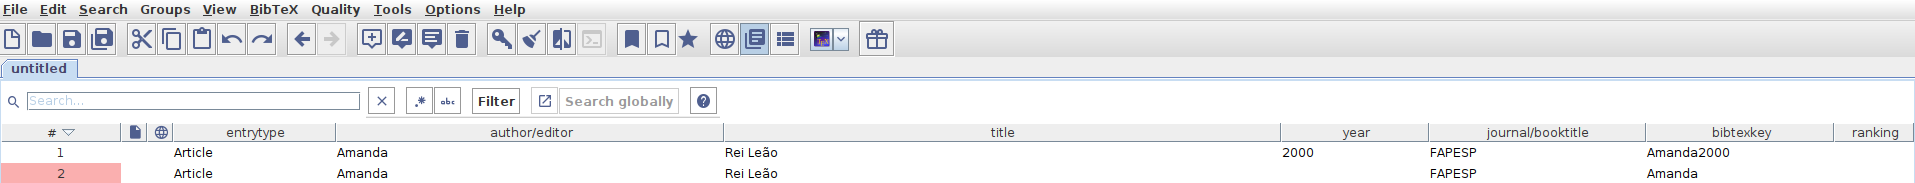
\includegraphics[width=15cm]{images/base_testes_article.png}
        \label{figura:base_testes_article}
    \end{figure}
        
        No entanto, vale ressaltar que o \textit{JabRef} considera como válidas quaisquer entradas com ao menos um caracter, como observado na figura \ref{figura:base_testes_article_caracter}:

    \begin{figure}[H]
        \caption{Entrada com apenas um caracter}
        \vspace{0.5cm}
        \centering
        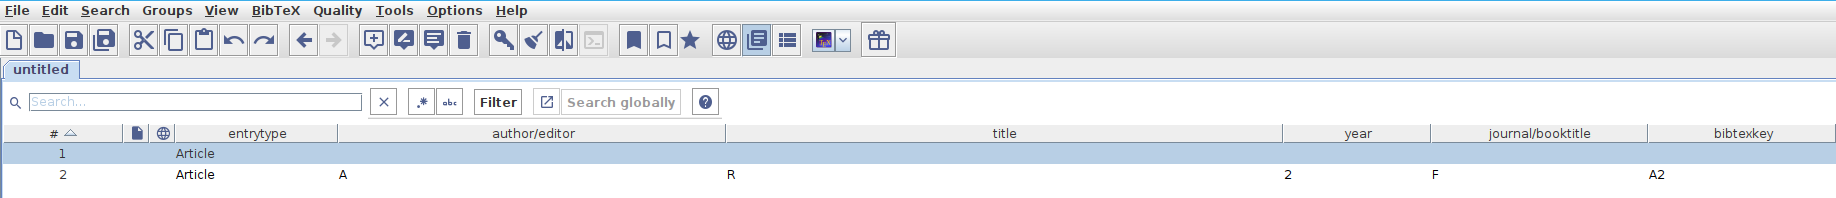
\includegraphics[width=15cm]{images/base_testes_article_caracter.png}
        \label{figura:base_testes_article_caracter}
    \end{figure}

        Verifica-se, então, que é possível adicionar entradas com anos menores que o ano atual. Outra saída válida, embora não seja esperado do programa, é a saída para entradas como anos posteriores ao ano atual, como o ano 20000. A figura \ref{figura:base_testes_article_ano_invalido} exibe a saída no \textit{JabRef}:

    \begin{figure}[H]
        \caption{Saída considerada válida para ano inválido}
        \vspace{0.5cm}
        \centering
        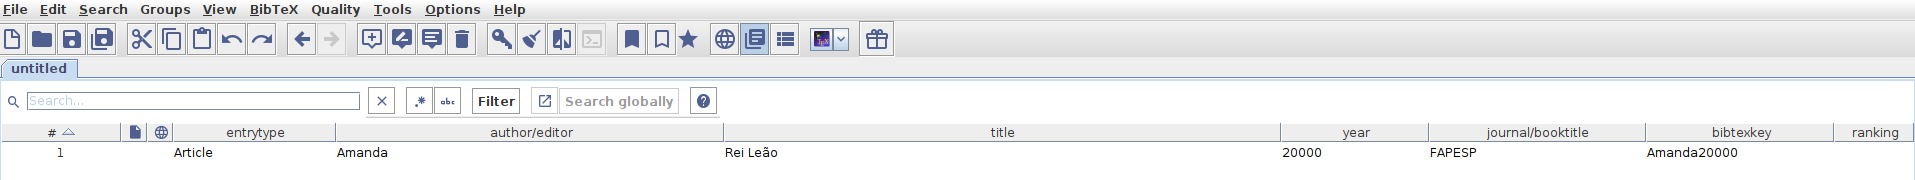
\includegraphics[width=15cm]{images/base_testes_article_ano_invalido.png}
        \label{figura:base_testes_article_ano_invalido}
    \end{figure}

        Um último exemplo de saída válida não esperada é a inserção de letras no campo \textit{Year}, como verificado na imagem \ref{figura:base_testes_article_ano_caracter}:

    \begin{figure}[H]
        \caption{Saída considerada válida para ano composto por letra}
        \vspace{0.5cm}
        \centering
        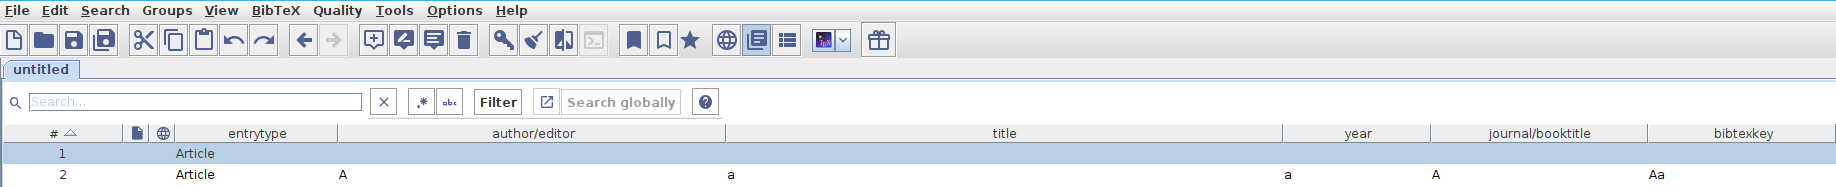
\includegraphics[width=15cm]{images/base_testes_article_ano_caracter.png}
        \label{figura:base_testes_article_ano_caracter}
    \end{figure}

        Desse modo, foi possível criar a tabela de testes representada pela figura \ref{figura:tabela_artigo}, que funciona de forma equivalente a uma tabela-verdade, visto ser necessário apenas preencher todos os campos requeridos - \textit{Author},\textit{Title}, \textit{Journal} e \textit{Year} - com ao menos um caracter para que a saída seja considerada válida pelo \textit{JabRef}.

    \begin{figure}[H]
        \caption{Tabela de testes funcionais para inserção em \textit{Article}}
        \vspace{0.5cm}
        \centering
        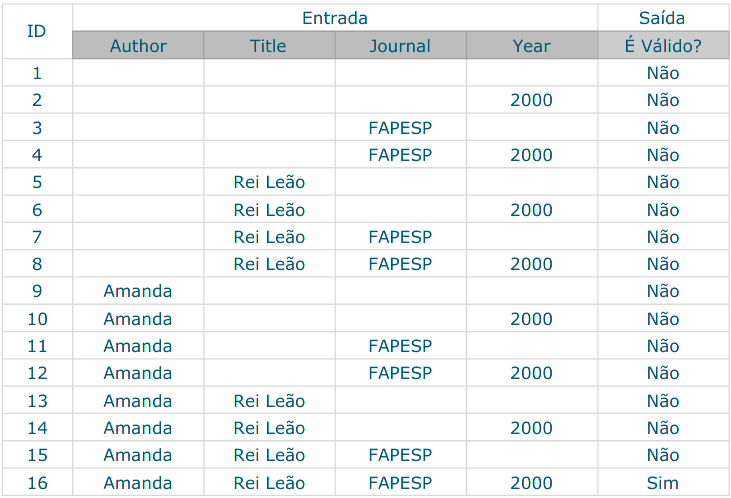
\includegraphics[width=15cm]{images/tabela_artigo.png}
        \label{figura:tabela_artigo}
    \end{figure}

    \subsection{Inserção de item bibliográfico - \textit{Book}}
        De forma análoga à inserção de item bibliográfico para \textit{Article}, foi construída uma tabela de testes para \textit{Book} que resultou na figura \ref{figura:tabela_livro_1}:
        \par As diferenças entre \textit{Book} e \textit{Article} são a quantidade e os campos de entrada. Ainda assim, para que o \textit{JabRef} resulte em saída válida, basta que todos os cinco campos de entrada - \textit{Title}, \textit{Publisher}, \textit{Year}, \textit{Author} e \textit{Editor} sejam preenchidos com ao menos um caracter.
    
    \begin{figure}[H]
        \caption{Tabela de testes funcionais para inserção em \textit{Book}}
        \vspace{0.5cm}
        \centering
        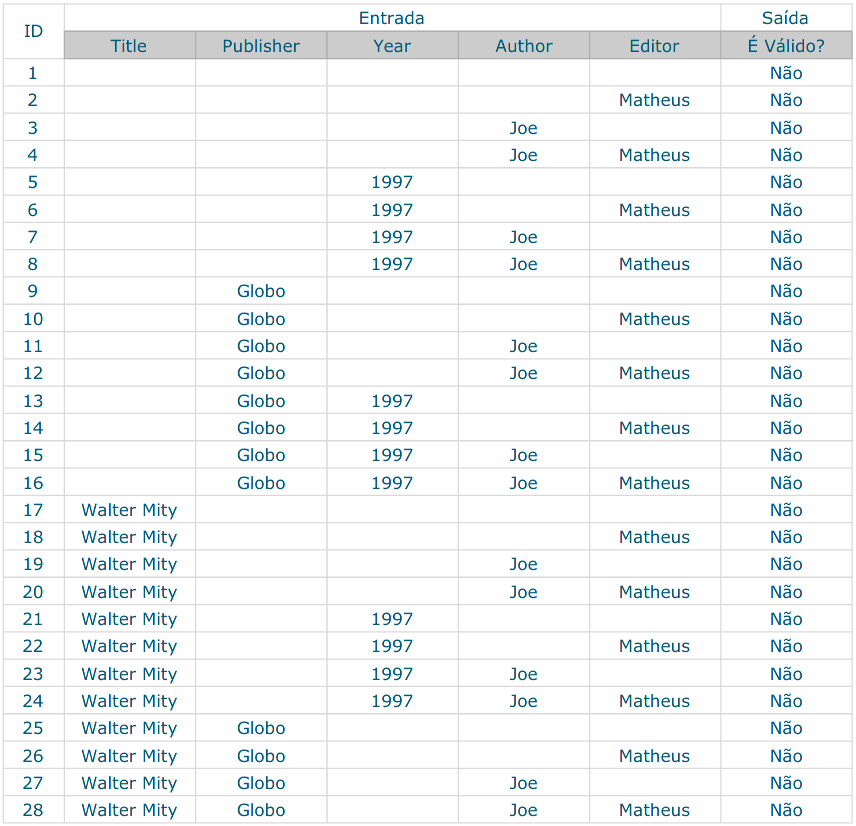
\includegraphics[width=15cm]{images/tabela_livro_1.png}
        \label{figura:tabela_livro_1}
    \end{figure}

    \begin{figure}[H]
        %\vspace{0.5cm}
        \centering
        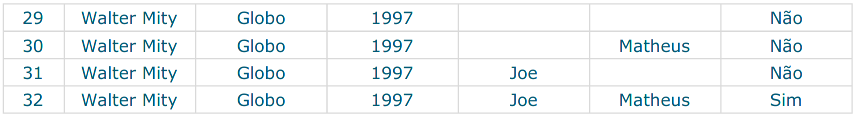
\includegraphics[width=15cm]{images/tabela_livro_2.png}
        \label{figura:tabela_livro_2}
    \end{figure}

    \subsection{Importação de itens bibliográficos}
        Os testes manuais realizados a respeito da importação de itens bibliográficos incluíram tanto a modificação do formato do arquivo a ser importado quanto a sintaxe deste, válida ou não.
        \par Para arquivos \textit{.bibtex} com sintaxe válida, como mostrado na figura \ref{figura:exemplo_importacao}, a importação ocorre com sucesso.
    
    \begin{figure}[H]
        \caption{Importação válida}
        \vspace{0.5cm}
        \centering
        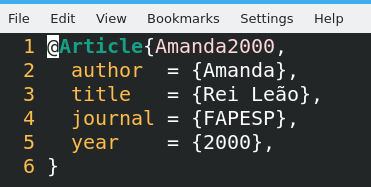
\includegraphics[width=8cm]{images/exemplo_importacao.png}
        \label{figura:exemplo_importacao}
    \end{figure}

        Ao testar a importação de arquivo \textit{.bibtex} com sintaxe inválida, mais especificamente com excesso de \textit{\}}, obteve-se sucesso ao importar o arquivo. O próprio \textit{JabRef} desconsiderou o \textit{\}} a mais.
    
    \begin{figure}[H]
        \caption{Importação com sucesso e sintaxe inválida}
        \vspace{0.5cm}
        \centering
        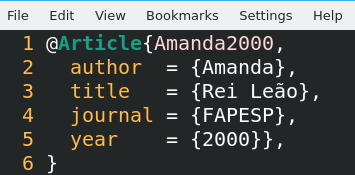
\includegraphics[width=8cm]{images/exemplo_importacao_valida.png}
        \label{figura:exemplo_importacao_valida}
    \end{figure}

    \begin{figure}[H]
        \caption{Resultado no \textit{JabRef}}
        \vspace{0.5cm}
        \centering
        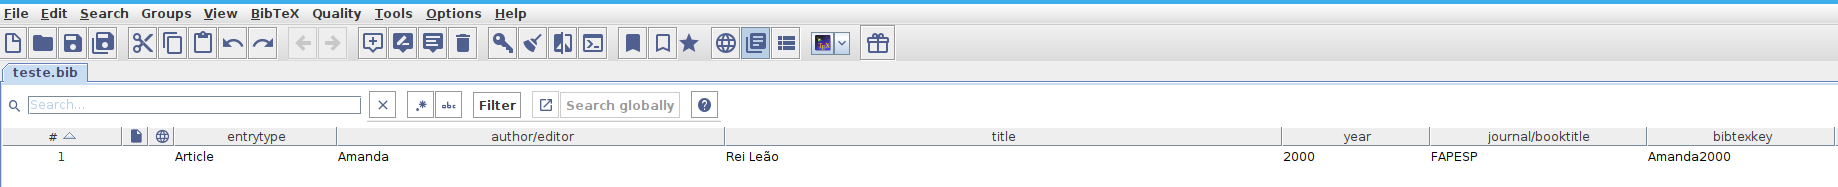
\includegraphics[width=15cm]{images/importacao_valida.png}
        \label{figura:importacao_valida}
    \end{figure}

        No entanto, a importação de arquivo \textit{.bibtex} com falta de \textit{\}}, como mostrado na figura \ref{figura:exemplo_importacao_valida}, resulta em falha.

    \begin{figure}[H]
        \caption{Importação com erro e sintaxe inválida}
        \vspace{0.5cm}
        \centering
        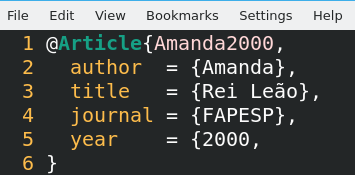
\includegraphics[width=8cm]{images/exemplo_importacao_invalida.png}
        \label{figura:exemplo_importacao_invalida}
    \end{figure}

        Não é possível importar arquivos com extensão inválida, como é o caso dos arquivos \textit{.csv}.
        \newline
        \par Portanto, obteve-se a tabela representada pela figura \ref{figura:tabela_importacao}:
    
    \begin{figure}[H]
        \caption{Tabela de testes funcionais para importação de itens bibliográficos}
        \vspace{0.5cm}
        \centering
        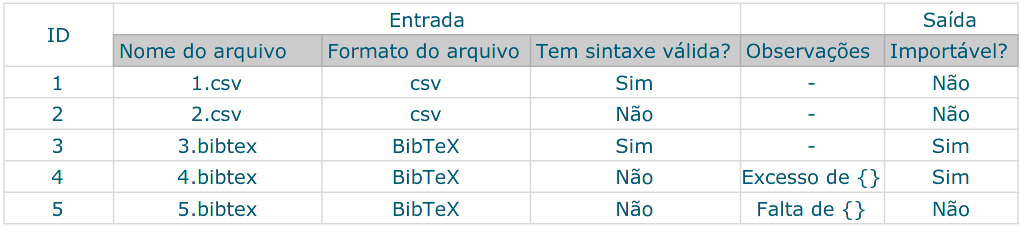
\includegraphics[width=15cm]{images/tabela_importacao.png}
        \label{figura:tabela_importacao}
    \end{figure}
